\section{P, NP and NPC.}

\subsection{Disposition}

\begin{enumerate}
 \item \textbf{Def. Problemer, Sprog, Encoding \& Stand-in Sprog}
    \subitem Def. Beslutningsproblem
    \subitem Def. Sprog
    \subitem Encoding
    \subitem Stand-in sprog
    \subitem Optimization Stand-ins
 \item \textbf{Def. P, NP, NP-hard \& NPC}
    \subitem  Tegn!
 \item \textbf{Def. Polynomial time computable maps}
 \item \textbf{Def. Reduktioner}
    \subitem  Proposition 3: Transitivitet (med bevis)
    \subitem  Proposition 4: Nedadgående lukkethed af P (uden bevis)
 \item \textbf{Lemma 7:} \textit{Hvis $L_1 \in$ NP-hard og $L_1 \leq L_2$, så er $L_2 \in$ NP-hard}
    \subitem  Bevis.
 \item \textbf{Proposition 5:} \textit{Lad $L \in$ NP-hard. Hvis $P \neq NP$, så er $L \notin P$.}
    \subitem  Bevis.
 \item \textbf{Proposition 6:} \textit{Hvis $L \in NPC$, så er $L \in P$ hviss. $P=NP$}
    \subitem  Bevis
 \item \textbf{Theorem 9.4:} \textit{INDEPENDENT SET $\in$ NPC}
    \subitem Vis 3SAT $\leq$ INDEPENDENT SET.
\end{enumerate}

\subsection{Emne detaljer}

Følgende afsnit indeholder detaljer om hvert punkt i dispositionen ovenfor (og muligvis flere ting også).

\subsubsection{Def. Problemer, Sprog, Encoding \& Stand-in Sprog}

Lad os starte med lige at få nogle grundlæggende definitioner og koncepter på plads. 

\paragraph{Def. Beslutningsproblem}
~\\
~\\
Vi fokuserer på såkaldte beslutningsproblemer hvor output altid er ''yes`` eller ''no``. Input her er så probleminstanser givet ved binære strenge. Altså strenge over $\left\lbrace 0,1 \right\rbrace$.

\paragraph{Def. Sprog}
~\\
~\\
Et givent problem, kan så modeleres som et sprog $L \subseteq \left\lbrace 0,1 \right\rbrace^*$ hvor medlemmerne af sproget er de instanser for hvilket output er ''yes`` og ikke-medlemmerne er de instanser hvor hvilket output er ''no``.

\paragraph{Encoding}
~\\
~\\
Vi sætter som sagt den ''restriktion`` at input er bitstrenge på $\left\lbrace 0,1 \right\rbrace^*$. Det er dog ikke en reel begrænsning, da reele computere alligevel gør selv samme med alt data gemt derpå. Således kan ethvert ''naturligt`` dataformat encodes som binært, således selv ASCII og UNICODE encodes nemt.
Dog er der selvfølgelig ting som selv en reel computer ikke kan encode korrekt i alle tilfælde, så som reele tal.

\paragraph{Stand-in sprog}
~\\
~\\
Hvis vi har et problem, for hvilket output ikke direkte kan beskrives som ''yes`` eller ''no``, men i stedet bør være en arbitrær bitstreng. Så konstruerer vi i stedet et såkaldt ''stand-in'' sprog. 

Et ``stand-in'' sprog $L_f$ repræsenterer så en given funktion $f: \left\lbrace 0,1 \right\rbrace^* \rightarrow \left\lbrace 0,1 \right\rbrace^*$ således:

\begin{align*}
 L_f &= \left\lbrace \left\langle x, b(j), y \right\rangle | f(x)_j = y \right\rbrace
\end{align*}
Hvor:\\
~\\
$x \in \left\lbrace 0,1 \right\rbrace^*$ \\
$j \in N$ \\
$y \in \left\lbrace 0,1 \right\rbrace$ \\

Og hvor $b(j)$ betyder den binære encodning af $j$. 

Her har vi, at $L_f$ har en effektiv algoritme, hvis og kun hvis, $f$ har det. Man skal så forstå ovenstående som, at output udregnes en bit af gangen.

\paragraph{Optimization Stand-ins}
~\\
~\\
Ligesom for arbitrære funktioner på bitstrenge, så skal vi også kunne modellere optimeringsproblemer. Lad os antage vi har fået følgende beskrivelse af et optimeringsproblem:

\begin{quotation}
 \textbf{OPT:} ``Givet en inputstreng der definerer et sæt mulige løsninger $F$ og en objective funktion $f$, find $x \in F$ der maksimerer $f(x)$''.
\end{quotation}

Dette kan vi så udtrykke som et beslutningsproblem ved blot at lave en lille ændring.

\begin{quotation}
 \textbf{OPT:} ``Givet en inputstreng der definerer $F$, $f$ og en target værdi $v \in Q$, bestem hvorvidt der er en løsning $x \in F$ således $f(x) \geq v$.''.
\end{quotation}

Det er dog ikke en perfekt ``stand-in'', da $L_{OPT}$ f.eks. godt kan være nem at løse uden at $OPT$ er det. Omvendt så hvis $L_{OPT}$ er svær at løse, så ved vi også $OPT$ er det. Det er således ikke muligt at bruge denne form for ``stand-in'' til at vise et givet problem er nemt at løse, men vi kan bruge det til at argumentere for et givent problem er svært.


\subsubsection{Def. P, NP, NP-hard \& NPC}

Lad os nu kigge på de kompleksitetsklasser vi har arbejdet med her i kurset.
\begin{center}
 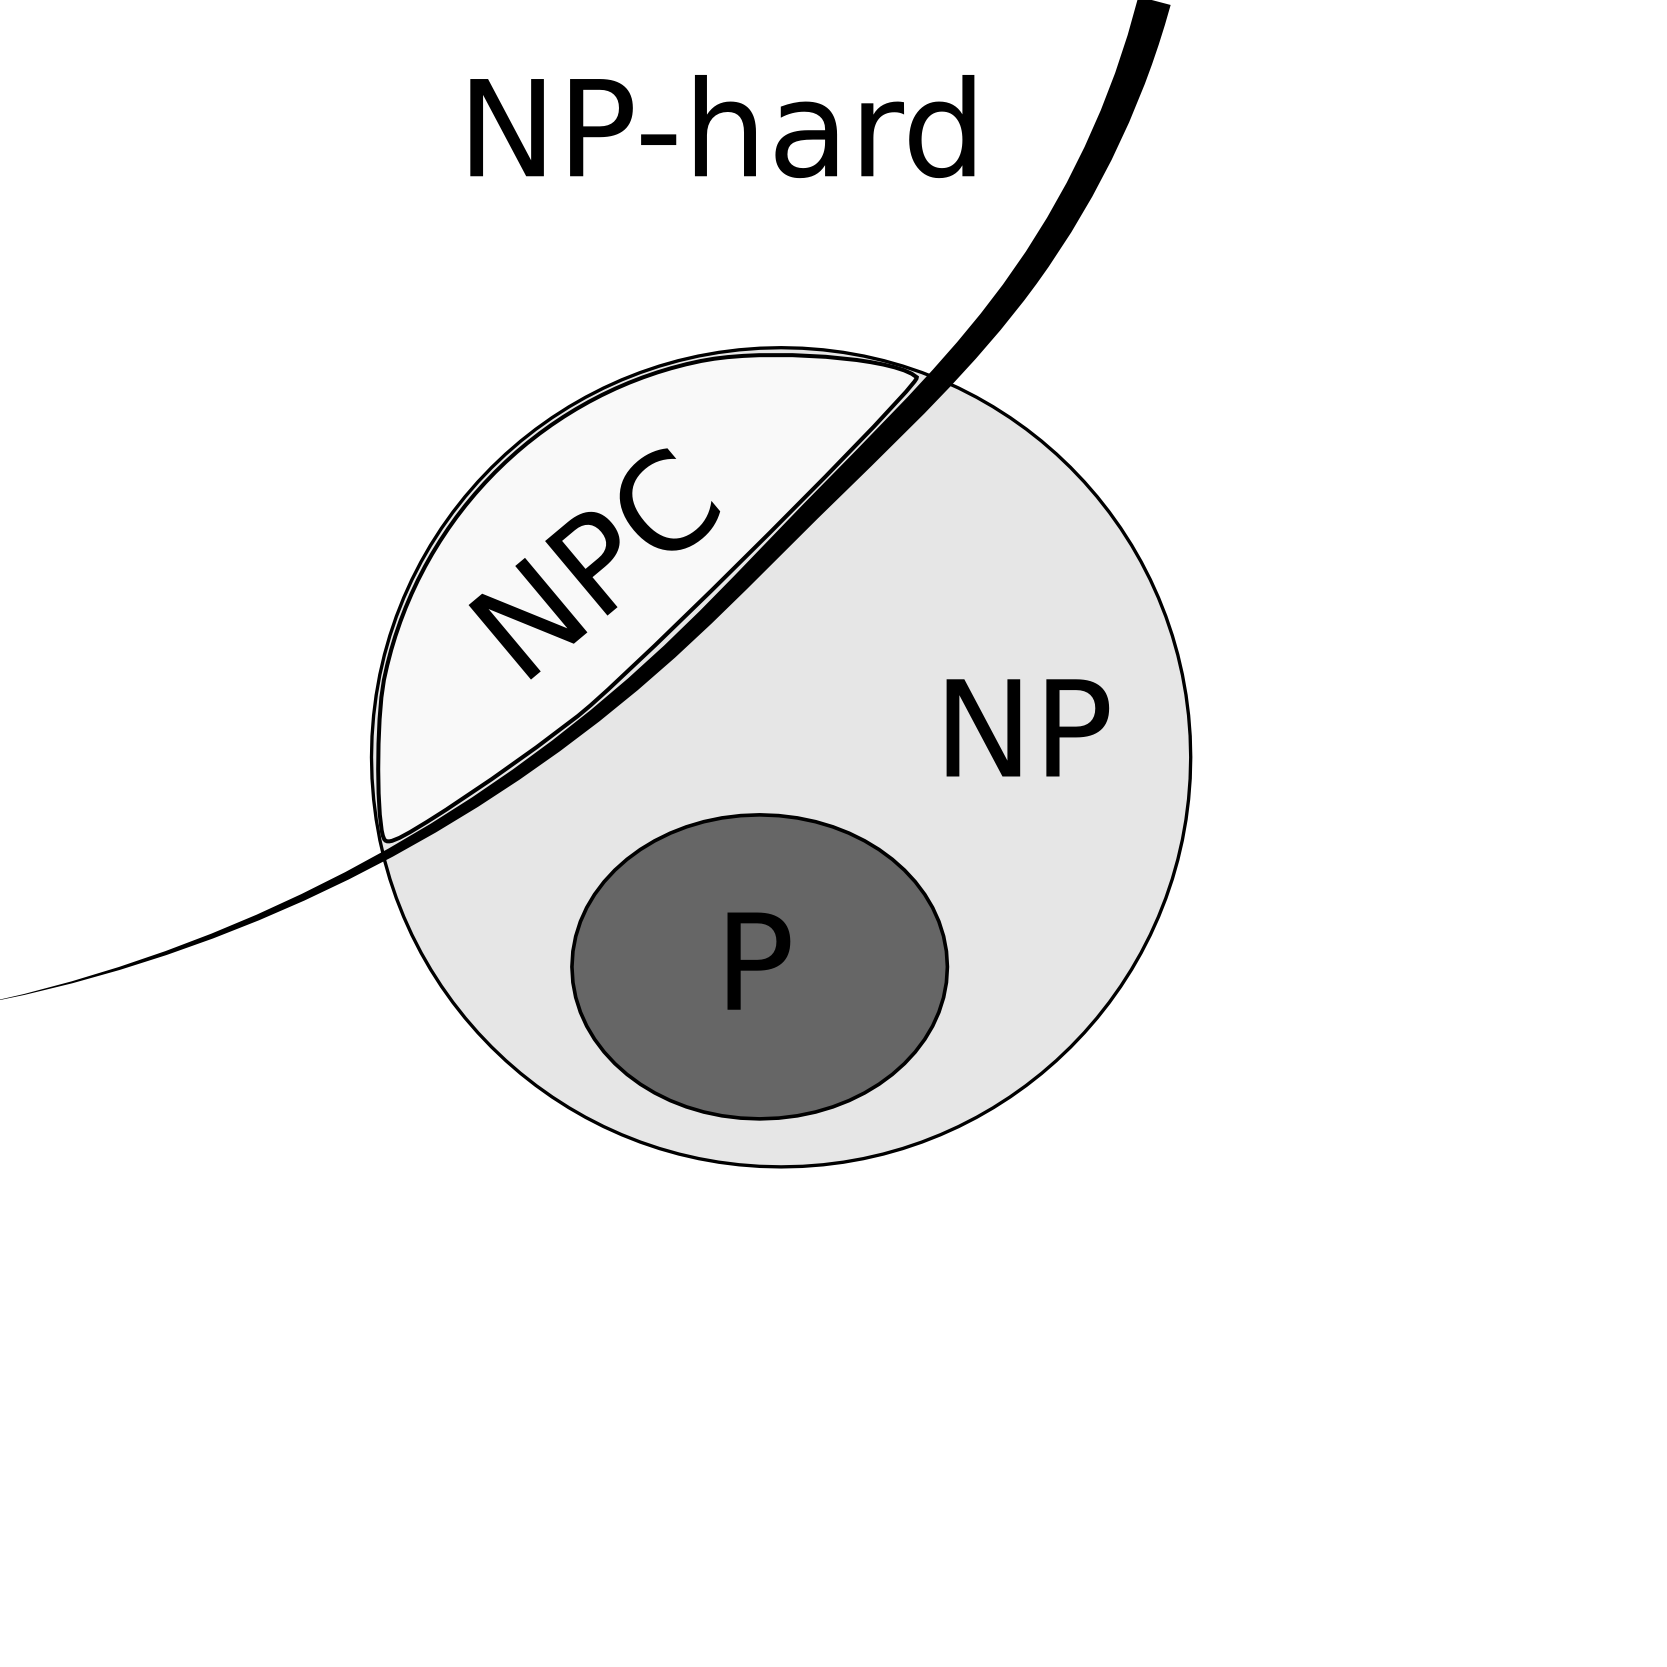
\includegraphics[bb=0 0 400 400,scale=0.3]{./PNPNPC.png}
 % PNPNPC.png: 1667x1667 pixel, 300dpi, 14.11x14.11 cm, bb=0 0 400 400
\end{center}


\paragraph{P}
~\\
~\\
Kompleksitetsklassen $P$ er formelt defineret således:
\begin{align*}
 P = \left\lbrace L \subseteq \left\lbrace 0,1 \right\rbrace^* | \exists \text{ TM } M_L \text{ der afgører L i polynomiel tid } \right\rbrace
\end{align*}
Altså klassen af beslutningsproblemer der kan blive bestemt af en deterministisk Turing Maskine hvor antallet af ``steps'' maskinen udfører for et givent $x$ maksimalt er $\rho(x)$ for et givent polynomiel $\rho$.\\
 
Intuivit ser vi kompleksitetsklassen $P$ som en klasse for problemer for hvilket vi kender en effektiv løsning. Altså ethvert problem med worst-case kørselstid på formen $O(n^k)$ for et givent $k$.

At worst-case kørseltid på et problem er polynomiel betyder dog ikke reelt at det er et nemt problem (modsat hvad Cobham's Thesis påstår). I hele den analyse ignorerer vi fuldkommen konstanter, samt forventet kørselstid som I mange tilfælde kan få ``sværere'' problemer til at køre bedre end ``nemme'' problemer i $P$.


\paragraph{NP}
~\\
~\\
Kompleksitetsklassen $NP$ er lidt mere kluntet formelt defineret, så vi starter lige med intuitionen først.

Intuitivt kan $NP$ ses som klassen af beslutningsproblemer for hvilket ``yes'' instanserne kan verificeres i polynomiel tid på en deterministisk Turing Maskine. Altså er det komplekse problemer med eksponentiel løbetid, men hvor løsningen til et sådant problem nemt kan verificeres til at være korrekt.\\
~\\
Kompleksitetsklassen $NP$ er formelt defineret således:
\begin{align*}
 NP = \left\lbrace L \subseteq \left\lbrace 0,1 \right\rbrace^* | \exists \rho \in Z[x], L' \in P, \forall x \in \left\lbrace 0,1 \right\rbrace^* : ( x \in L \Leftrightarrow \exists y \in \left\lbrace 0,1 \right\rbrace^* : |y| \leq \rho(|x|) \wedge \left\langle x,y \right\rangle \in L') \right\rbrace
\end{align*}
Definitionen skal forståes således: Vi har et sprog $L' \in P$, samt et polynomiel $\rho$. Vi tænker så nu på et sæt af binære strenge af længde maksimalt $\rho(|x|)$, hvor disse representerer mulige løsninger til probleminstansen $x$. Med denne fortolkning bliver $\left\langle x,y \right\rangle \in L'$ så måden hvorpå vi tester om en given løsning $y$ virkelig er en korrekt løsning. 

Denne form for søgningsproblem kaldes ofte for et simpelt søgningsproblem, da den kan verificeres i polynomiel tid, men ikke løses deri (antaget $P \neq NP$).\\

For at løse et givent NP problem kunne vi så løbe igennem alle mulige løsninger for $y$, som sammenlagt ville være $2^{\rho(|x|)+1}-1$, og for hver af dem tjekke $\left\langle x,y \right\rangle \in L'$. Det ønsker vi dog ikke, da det ville tage eksponentiel tid. I stedet forsøger man ofte at finde snedige måder at lave speed-ups og/eller lave approximationsalgoritmer af forskellige art.

Og i visse tilfælde er man også heldig at finde en algoritme i $P$ for et $NP$ problem, hvorved man har vist at problemet i virkeligheden ligger i $P$ som jo er et subset af $NP$.

\paragraph{NP-hard}
~\\
~\\
Et sprog defineres som NP-hard såfremt der gælder:

\begin{align*}
 \forall L' \in NP: L' \leq L
\end{align*}

Altså gælder der, at ethvert sprog $L'$ i NP kan reduceres til $L$. Intuitionen er her, at algoritmen til at løse NP-hard problemet er så stærk (eller generel) at den kan bruges til at løse ethvert andet problem i NP. Man siger desuden, at et NP-hard problem således er mindre sandsynlig end noget andet sprog i NP, til at være i P.\\

Navnet kan dog være lidt forvirrende, da et NP-hard problem faktisk ikke behøver være i NP og hvis de er, så kaldes de faktisk ikke engang bare NP-hard længere.

\paragraph{NPC}
~\\
~\\
NP-Complete (NPC) er den særlige klasse af problemer der både er NP-hard og befinder sig i NP. Formelt defineret således: 

\begin{align*}
 NPC = \left\lbrace L \in \left\lbrace 0,1 \right\rbrace^* | L \in NP \wedge (\forall L' \in NP: L' \leq L) \right\rbrace
\end{align*}

NPC problemer er særligt interessante, da vi kan bruge dem til at bevise et givent problem er NP-Complete, således vi ikke spilder tid på forsøg med at finde en algoritme i $P$ for problemet (antaget $P\neq NP$). Dette gør vi vha. noget vi kalder reduktioner, som bygger på polynomial time computable maps.

\subsubsection{Def. Polynomial time computable maps}

Et polymial time computable map er en funktion $f: \left\lbrace 0,1 \right\rbrace^* \rightarrow \left\lbrace 0,1 \right\rbrace^*$ hvor der, for en given polynomiel $\rho$ gælder:

\begin{align*}
 &\forall x: |f(x)| \leq \rho(|x|) \\
 &L_f	 \in P
\end{align*}

Altså at længden af funktionens output skal være polynomielt på alle input og ``stand-in'' beslutningsproblemet $L_f$ tilknyttet $f$ skal være i P. Man kan se polynomial time computable maps som en måde at oversætte en given repræsentation eller modellering til en anden i polynomiel tid vha. en oversættelsesfunktion $f$.

\subsubsection{Def. Polynomielt ækvivalente representationer}

Et sted polynomial time computable maps bruges er ved objekt-repræsentationer.

En repræsentation af objekter (grafer, numre, etc.) som strenge kaldes ``god'' såfremt sproget af lovlige repræsentationer heraf er i P. Man kalder så to repræsentationer polynomielt ækvivalente såfremt der kan oversættes imellem dem vha. et polynomial time computable map.


\subsubsection{Def. Reduktioner}

Det bringer os så til en grundlæggende metode i computationel kompleksitetsteori, nemlig reduktioner. Først og fremmest den formelle definition.

Givet to sprog $L_1$ og $L_2$, en polynomiel reduktion $r$ af $L_1$ til $L_2$ er en polynomial time computable map for hvilken der gælder:

\begin{align*}
 \forall x : x \in L_1 \text{ hviss. } r(x) \in L_2
\end{align*}

Dette skrives som $L_1 \leq L_2$, hvor man læser det som at $L_1$ reduceres til $L_2$. Intuitivt betyder reduktion blot, at vi kan oversætte enhver given instans af $L_1$ til en anden instans af $L_2$. Vi siger desuden, at $L_2$ er et mere generelt sprog end $L_1$ og kan derfor ses, som værende mere sandsynlig til ikke at være i $P$.


Herudover har  reduktioner desuden to nyttige egenskaber vi skal bruge senere.

\paragraph{Proposition 3: Hvis $L_1 \leq L_2$ og $L_2 \leq L_3$, så gælder der $L_1 \leq L_3$}
~\\
~\\
Denne proposition underbygger, at reduktioner er transitive. Vi beviser den således:

\begin{proof}
 Vi har polynomial time computable maps $r_1()$ og $r_2()$, hvor følgende ting gælder:

\begin{itemize}
 \item For ethvert $x$ gælder der, at $x \in L_1$ hvis og kun hvis $r_1(x) \in L_2$.
 \item For ethvert $y$ gælder der, at $y \in L_2$ hvis og kun hvis $r_2(y) \in L_3$.
\end{itemize}

Således har vi for alle $x$, at $x \in L_1$ hvis og kun hvis $r_2(r_1(x)) \in L_3$. Og siden vi blot har brugt to polynomial time computable maps efter hinanden (hvormed det hele kan ses som en polynomial time computable map), så har vi $L_1 \leq L_3$.
\end{proof}

\paragraph{Proposition 4: Hvis $L_1 \leq L_2$ og $L_2 \in P$, så er $L_1 \in P$.}

Proposition 4 siger intuitivt, at $P$ er lukket nedad under reduktion. 


\subsubsection{Lemma 7}

For at kunne bevise et givent sprog er NP-hard, så bruger vi  polynomielle reduktioner fra kendte NP-hard problemer, fremfor at forsøge et direkte bevis. For at kunne lave disse reduktioner, så har vi brug for følgende lemma.\\
~\\
\textbf{Lemma 7:} Hvis $L_1$ er NP-hard og $L_1 \leq L_2$ så er $L_2$ også NP-hard.

\begin{proof}
 Siden $L_1$ er NP-hard, så ved vi alle sprog $L$ i NP kan reduceres til det ($\forall L \in NP: L \leq L_1$). Så når $L_1 \leq L_2$, så kan vi bruge transitivitetsreglen (Proposition 3) og konkludere at ethvert sprog $L$ reducerer til $L_2$ ($\forall L \in NP: L \leq L_1 \leq L_2$), hvormed $L_2$ altså er NP-hard.
\end{proof}


\subsubsection{Proposition 5}

Som sagt, så er NP-hard problemer de problemer der intuitivt er mindst sandsynlige til at befinde sig i P. Faktisk kan vi udtrykke det som følgende proposition:\\
~\\
\textbf{Proposition 5:} Lad $L$ være et NP-hard sprog. Hvis $P \neq NP$ så er $L \notin P$.

\begin{proof}
 Denne proposition kan bevises ganske simpelt. 

Siden $L$ er NP-hard ved vi, at følgende gælder:

\begin{align*}
 \forall L' \in NP : L' \leq L
\end{align*}

Altså at alle andre sprog $L'$ i NP reducerer til $L$.

Hvis vi derfor antager, at $L \in P$, så fordi $P$ er lukket under reduktion (jvf. Proposition 4), så er alle $L' \in NP$ også i $P$, hvorved $P=NP$. \\

Vi har derfor, at hvis $L \in$ NP-hard og $P \neq NP$, så er $L \notin P$.

\end{proof}


\subsubsection{Proposition 6}

Som sagt er det ikke alle NP-hard sprog der ligger i NP, men vi er specielt interesseret i dem der gør, nemlig NPC sprogene.\\
~\\
\textbf{Proposition 6:} Lad $L \in NPC$. Så gælder der at $P=NP$ hvis og kun hvis $L \in P$.

\begin{proof}
 Denne proposition er om muligt endnu simplere. Fra Proposition 5 ved vi at $P=NP$ hvis $L \in P$, men vi ved ikke direkte herfra, at det er det eneste tilfælde hvor det gælder. 

Det ved vi derimod ud fra, at $L \in NP$. Hvis vi ser det fra begge sider så at sige, så ville $L \in P$ betyde at $P=NP$ og $P=NP$ ville betyde at $L \in P$.
\end{proof}

\subsubsection{Theorem 9.4}

Fordi emnet her mangler lidt dybde i kurset, så lad os gå videre og kigge på et grafproblem kaldet INDEPENDENT SET. Vi har en urettet graf $G=(V,E)$. Lad så $I \subseteq V$, hvor vi kalder $I$ ``independent'' hvis der for alle $i,j \in I$ ikke er en kant imellem $i$ og $j$. 

INDEPENDENT SET problemet er så: \textit{Givet en urettet graf $G=(V,E)$ og et mål $K$, er der et independent set $I$ hvor $|I|=K$?}\\
~\\
\textbf{Theorem 9.4:} INDEPENDENT SET $\in$ NPC

\begin{proof}
 For at kunne bevise INDEPENDENT SET er i NPC, så reducerer vi fra 3SAT. Vi skal bruge en lille gadget, nemlig en trekant som dem nedenfor. Begrundelsen for dette er, at hvis grafen indeholder en trekant, så ved vi på forhånd et independent set maksimalt kan indeholde 1 af de 3 knuder i trekanten. Dette bruger vi så i beviset ved at vi begrænser den mængde af grafer vi kigger på, til kun at tillade grafer vis knuder kan opdeles i $m$ disjunkte trekanter. Således får vi at vi maksimalt kan have et independent set af størrelse $m$ (en fra hver trekant) og at denne eksisterer hvis og kun hvis kanterne i konstruktionen tillader vi kan vælge en knude fra hver trekant.
 \begin{center}
 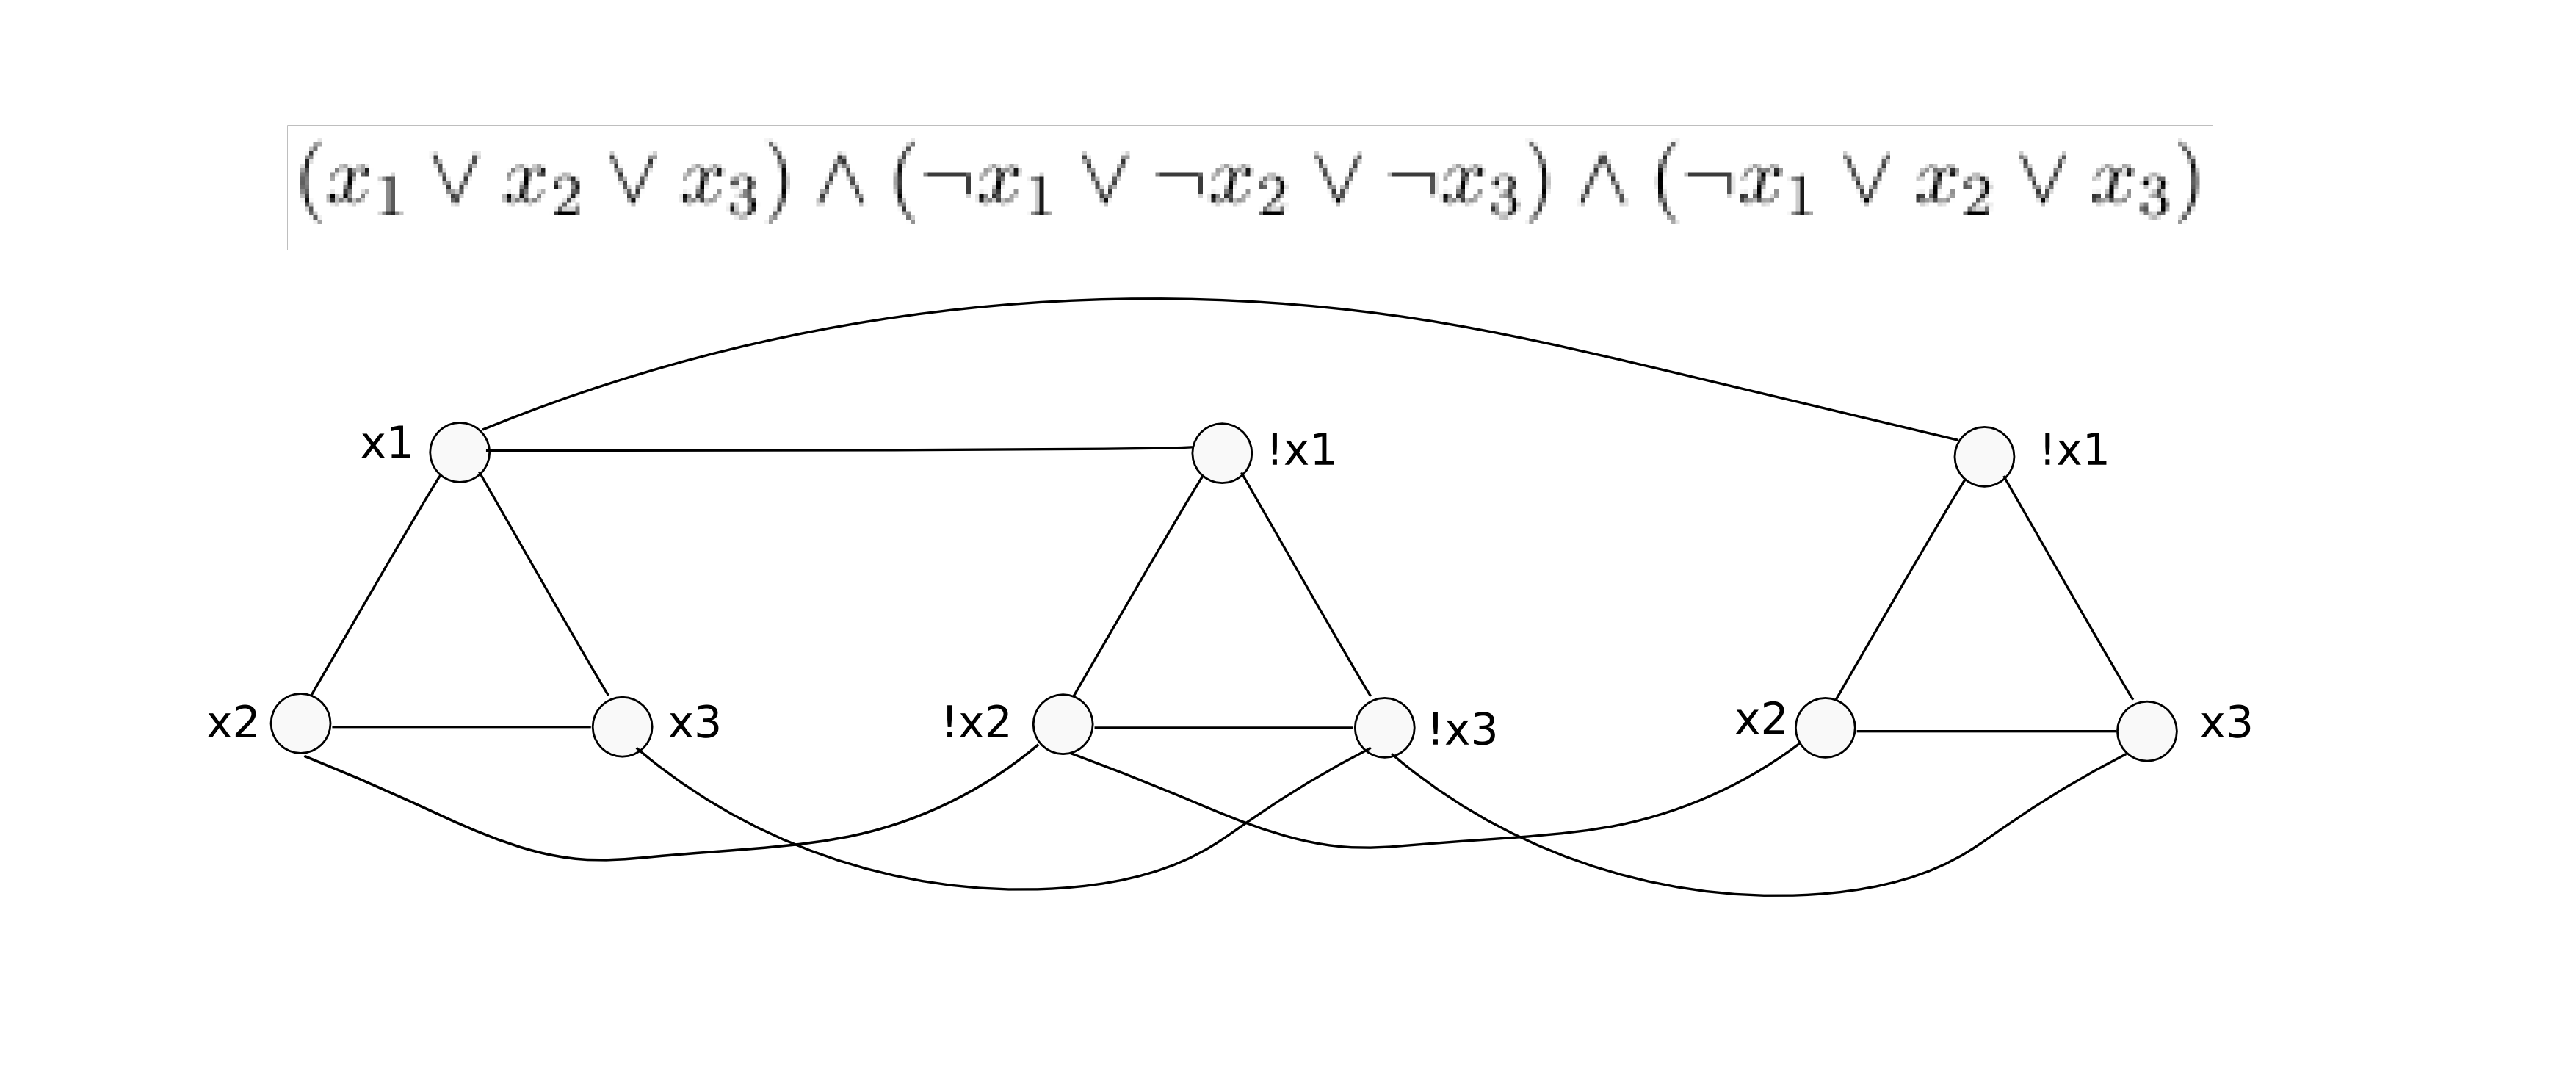
\includegraphics[bb=0 0 842 595,scale=0.5]{./INDEPENDENTSET.png}
 % INDEPENDENTSET.png: 3508x2480 pixel, 300dpi, 29.70x21.00 cm, bb=0 0 842 595
\end{center}
Konstruktionen i reduktionen fra en 3SAT instans til INDEPENDENT SET kommer så nemt heraf (illustreret ovenfor). Konstruktionen er som følger:

\begin{enumerate}
 \item For hver af de $m$ klausuler af en given CNF formel $f$ skabes en ny trekant i $G$.
 \item Hver knude i trekanten svarer så til en literal i den pågældende klausul.
 \item Tilføj kanter mellem nodes med modsatte literals (således $x_1$ får en kant til $\neg x_1$).
 \item Sæt målet $K$ i INDEPENDENT SET problemet til $m$.
\end{enumerate}

Herefter er konstruktionen færdig. Vi påstår så nu, at der er et independent set af $K$ nodes i $G$ hvis og kun hvis $f$ tilfredsstilles. Hvis vi antager sådan et independent set $I$ eksisterer, så siden $K=m$, så må $I$ indeholde en knude pr. trekant. Siden alle nodes er labeled med deres literal og $I$ ikke indeholder to knuder svarende til modsatte literals, så er $I$ en sandt/falsk tildeling der tilfredsstiller $f$. Alle literals indeholdt i $I$ bliver så dem der er ``true''.

Og set fra den anden side, så hvis vi ved $f$ har en tilfredstillende tildeling, så identificerer vi blot de literals der bliver ``true'' i $f$ og markerer dem som en del af $I$ i grafen $G$, hvorved vi får et independent set med $m=K$ uafhængige knuder.

Vi har derved bevist at 3SAT $\leq$ INDEPENDENT SET, hvorved vi kan konkludere INDEPENDENT SET $\in$ NPC.
\end{proof}